\documentclass{article}
\usepackage{verbatim}
\usepackage{url}
\usepackage{graphicx}
\usepackage{xspace}

\usepackage[pdftex, pdfpagemode=none, pdfstartview=FitH]{hyperref}
\hypersetup{
  pdfauthor = {Kurtis L. Nusbaum},
  pdftitle = {Evaluation of Tpetra's Matrix-Matrix Multiplication Routine},
  pdfkeywords = {multigrid, MueLu, Trilinos, software design, matrix matrix multiplication},
  colorlinks= {true},
  citecolor = {blue},
}

\usepackage[usenames]{color}
\definecolor{jhuGreen}{rgb}{0,.7,.4}
\newcommand{\JJH}[1]{\textcolor{jhuGreen}{JJH: #1}}

\newcommand{\mahts}[1]{\textsuperscript{#1}}
\newcommand{\Aprime}{\ensuremath{A'}\xspace}
\newcommand{\Bprime}{\ensuremath{B'}\xspace}
\title{Evaluation of Tpetra's Matrix-Matrix Multiplication Routine}
\author{Kurtis L. Nusbaum}
\date{August 2011}
\begin{document}
\maketitle

\begin{abstract}
Over the course of the last year, a matrix-matrix multiplication routine has been developed for the Tpetra package.
This routine is based the same algorithm that is used in EpetraExt with some heavy modifications. Since it 
achieved a working state, several major optimizations have been in an effort to speed up the routine. This paper will
discuss the optimizations made to the routine, its current state, and where future work needs to be done.
\end{abstract}
\clearpage
\tableofcontents
\clearpage

\section{Basic Outline of the Algorithm}
\JJH{I'd suggest adding citations throughout.}
The Tpetra matrix-matrix multiply algorithm allows two matrices ($A$ and $B$) to be multiplied. The result of this 
multiplication is then placed in a third matrix ($C$).
The basic algorithm is as follows:
\begin{enumerate}
  \item \Aprime and \Bprime are created from $A$ and $B$, respectively. If it has been specified that $A$ should be transposed, an actual 
  transpose of the matrix is created and assigned to \Aprime. Otherwise \Aprime is simply equals to $A$. The same is done for 
  creating \Bprime.
  \item A ``view'' of \Aprime and a ``view'' of \Bprime are created. These views provide fast access to information that 
  will be needed later in the algorithm. In addition, any importations of off-processor elements is done. Namely, all the 
  rows in \Bprime that contain columns needed by the local copy of \Aprime are imported.
  \item The sparsity pattern of $C$ is determined by doing a symbolic multiplication of \Aprime and \Bprime, i.e., no actual
  numeric computations are done. In this run, 
  column indices for $C$ are computed and used to construct a graph.
  \item The actual multiplication of \Aprime and \Bprime is done by iterating through each row of \Aprime. For each row in 
  \Aprime, every row in \Bprime is looped through and the appropriate calculations are done.
  \item Unless indicated otherwise by the user, \verb!fillComplete! is called on matrix $C$.
\end{enumerate}

\section{Optimization}

\section{Removal of Specific Transpose Mode Kernels}
In the original ExpetraExt algorithm there was actually a separate kernel for each possible transpose combination 
%(e.g. A\mahts{T}*B, A*B\mahts{T}, and A\mahts{T}*B\mahts{T}).
(e.g., $A^{T}B$, $AB^T$, and $A^TB^T$).
Some of these kernels relied on a function called \verb!find_rows_containing_columns!. The relevant things to know about this 
function is that one of its arguments was a matrix and during execution it created an array that was of size 
$N_c+ 2N_p + N_p N_r$, where
$N_c$, $N_p$, and $N_r$ are the number of columns, processors, and rows, respectively.
%$$\mbox{NumberOfColumns}+2\mbox{NumberOfProcessors}+\mbox{NumberOfProcessors}*\mbox{NumberOfRows}$$.
Obviously this is not scalable. At anything but the lowest processor counts, this array quickly balloons to a size that 
won't fit in memory. We decided to just remove this function and the specific transpose kernels. Tpetra has a very fast 
transposer that we now use instead. We take what ever the given matrices are, transpose them to the users specification, 
and then just use the regular $AB$ kernel. This has \emph{significant} performance benefits when doing operations like 
$A^TB$.

\subsection{Fixing FillComplete's Sort}
As part of its algorithm, the \verb!fillComplete! function relies on a function called sort2. This function performs a sort 
on two arrays by sorting the first array and concurrently doing the same permutations on the second array, 
i.e. both arrays are sorted according to the ordering of the first array. The main use case for this function is sorting 
an indices array and moving the values in a values array so that they stay matched up with their associated index.

Up until recently, the sort2 function relied on an insertion sort algorithm. We modified the function so that it first 
checks to see if the arrays are already sorted (which happens quite often) and returns right away if they are. 
If the arrays are not sorted, a quicksort is performed on the arrays.
\JJH{Can you quantify the difference in performance that just this change makes?}

\subsection{Streamlining the Graph Building Routine}
The original algorithm from EpetraExt used the same function for both building the graph of matrix $C$ and calculating its 
values by doing two passes through the function with different data. 
As a result, on the first pass through the function when the graph was being calculated, the values for matrix $C$ were also 
calculated, but thrown out. It's not until the second pass through the function 
that the values calculated are actually inserted into matrix $C$. We modified this function so that it
takes an argument which indicates whether or not we're just calculating the graph for matrix $C$. If we're just calculating 
the graph, all the value calculation is skipped.
\JJH{Can you quantify the difference in performance that just this change makes?}

\section{Performance}
We conducted a series of weak-scaling studies on the Hopper NERSC machine. Hopper is a Cray XE6 with 24 cores
per-node~\footnote{For more machine information regarding Hopper, please visit \url{http://www.nersc.gov/systems/hopper-cray-xe6}}.

\subsection{Comparison of Development Stages}
Figure~\ref{tpetracomptime} and Figure~\ref{tpetracompeff} show the test results of comparing the Tpetra matrix multiply 
routine at various stages of its 
development.  The tests were as such: Two matrices were constructed using a 3D Laplace stencil. Each node was assigned 
$110^3$ number of rows from each matrix. Then the two matrices were multiplied together. The multiplication is what 
we timed. We ran these experiments three times for each node count, and then averaged the results.
The red line represents the routine as it was when we first got the routine working. The blue line is from after 
we fixed the sort2 algorithm problem. And the purple line represents the routine after all optimizations had been applied.
As can be clearly seen, the optimizations we applied helped the algorithm substantially.

\begin{figure}
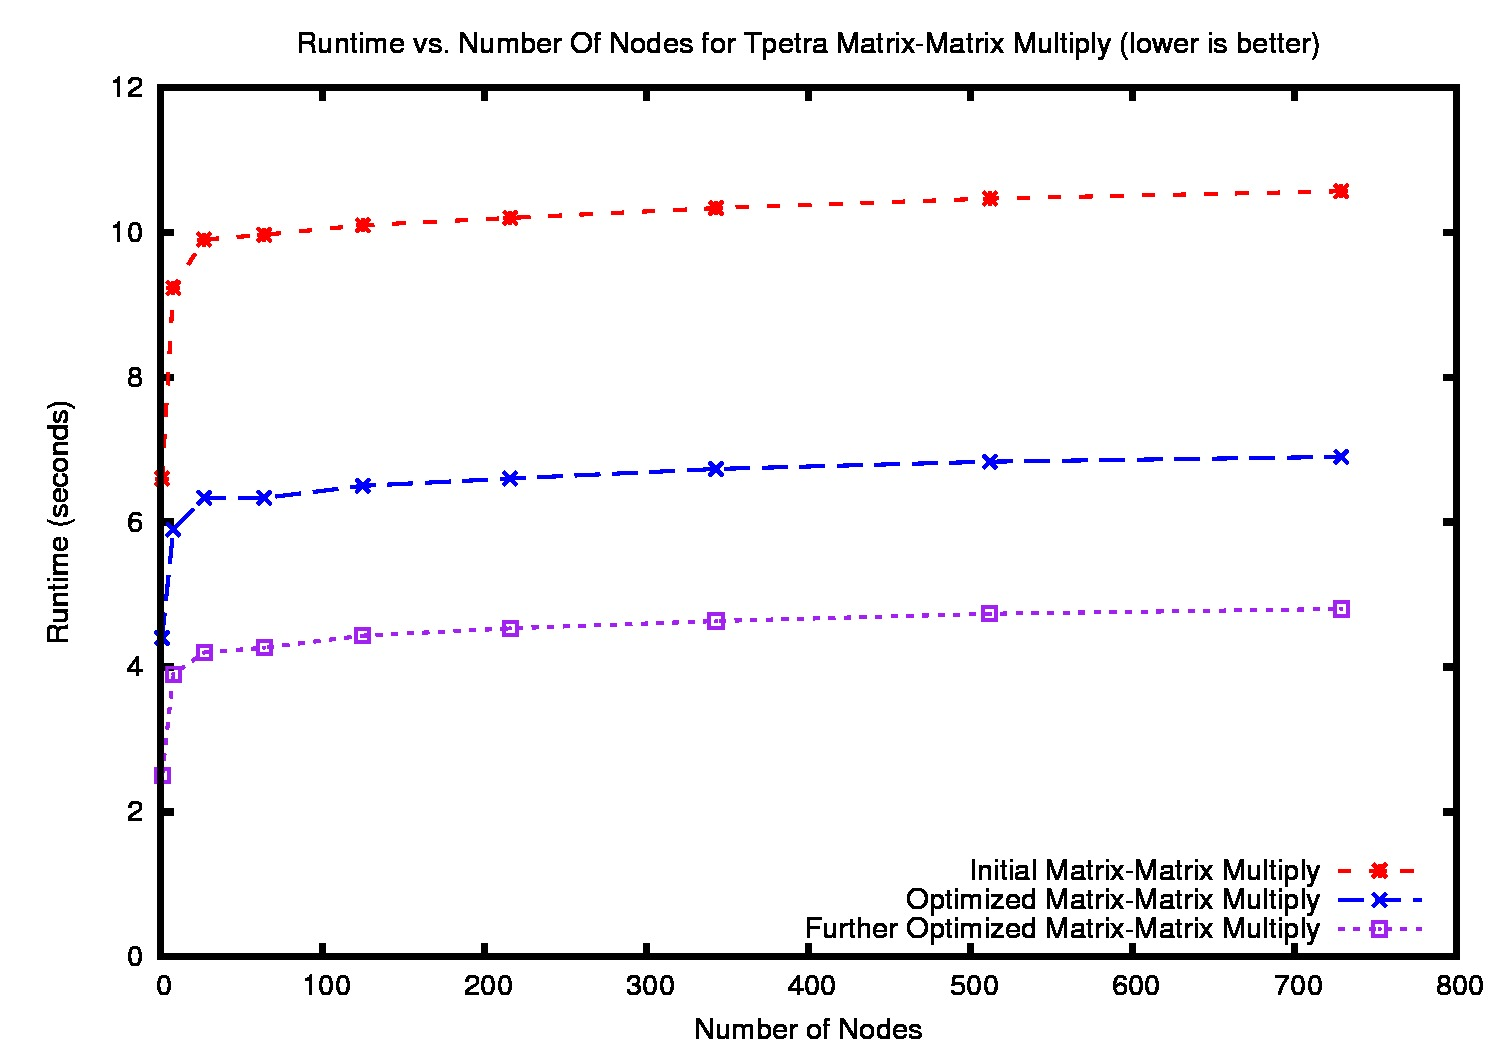
\includegraphics[scale=.4]{tpetratime.jpg}
\caption[Time Comparison]{A comparison of the Tpetra matrix multiply routine's runtime 
throughout various stages of its development}
\label{tpetracomptime}
\end{figure}

\begin{figure}
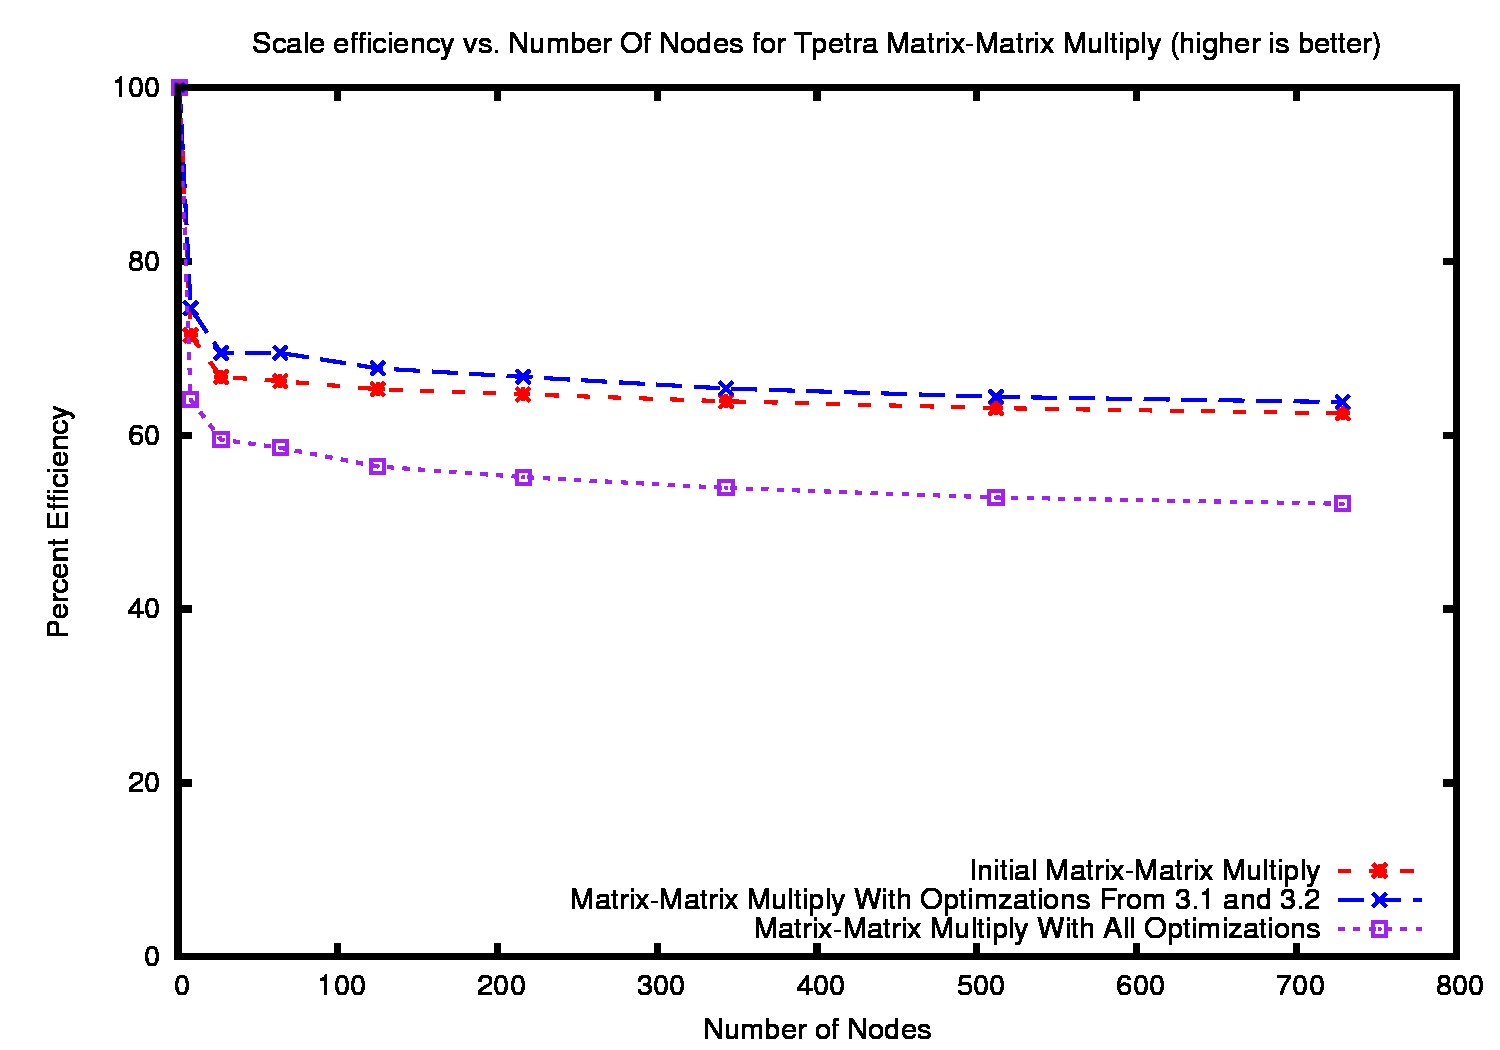
\includegraphics[scale=.4]{tpetraeff.jpg}
\caption[Efficiency Comparison]{A comparison of the Tpetra matrix multiply routine's scaling efficiency
throughout various stages of its development}
\label{tpetracompeff}
\end{figure}


\subsection{Tpetra vs. EpetraExt vs. ML}
Figure~\ref{totaltime} and Figure~\ref{totaleff} show the test results of comparing the Tpetra matrix multiply routine 
(with all of its optimizations) to the other matrix multiply routines in Trilinos (namely the original EpetraExt 
routine and two ML routines). These tests were conducted in the same manner as our development stages comparison. 
The encouraging thing about these results is that the Tpetra algorithm is as good as, if not better, than the EpetraExt 
algorithm at scale. It should be noted that the ML lines are cut short because at the next problem size in our testing, 
they would fail due to a memory error. Consequently, we could not run tests for greater problem sizes with ML. 
\JJH{Where did this memory error occur?  ML has been run on pretty big problems in the past ....}
It's also worth noting that in terms of efficiency, Tpetra seems to scale much better than all the rest.
\JJH{Scaling of ML appears to have the same trend.}

\begin{figure}
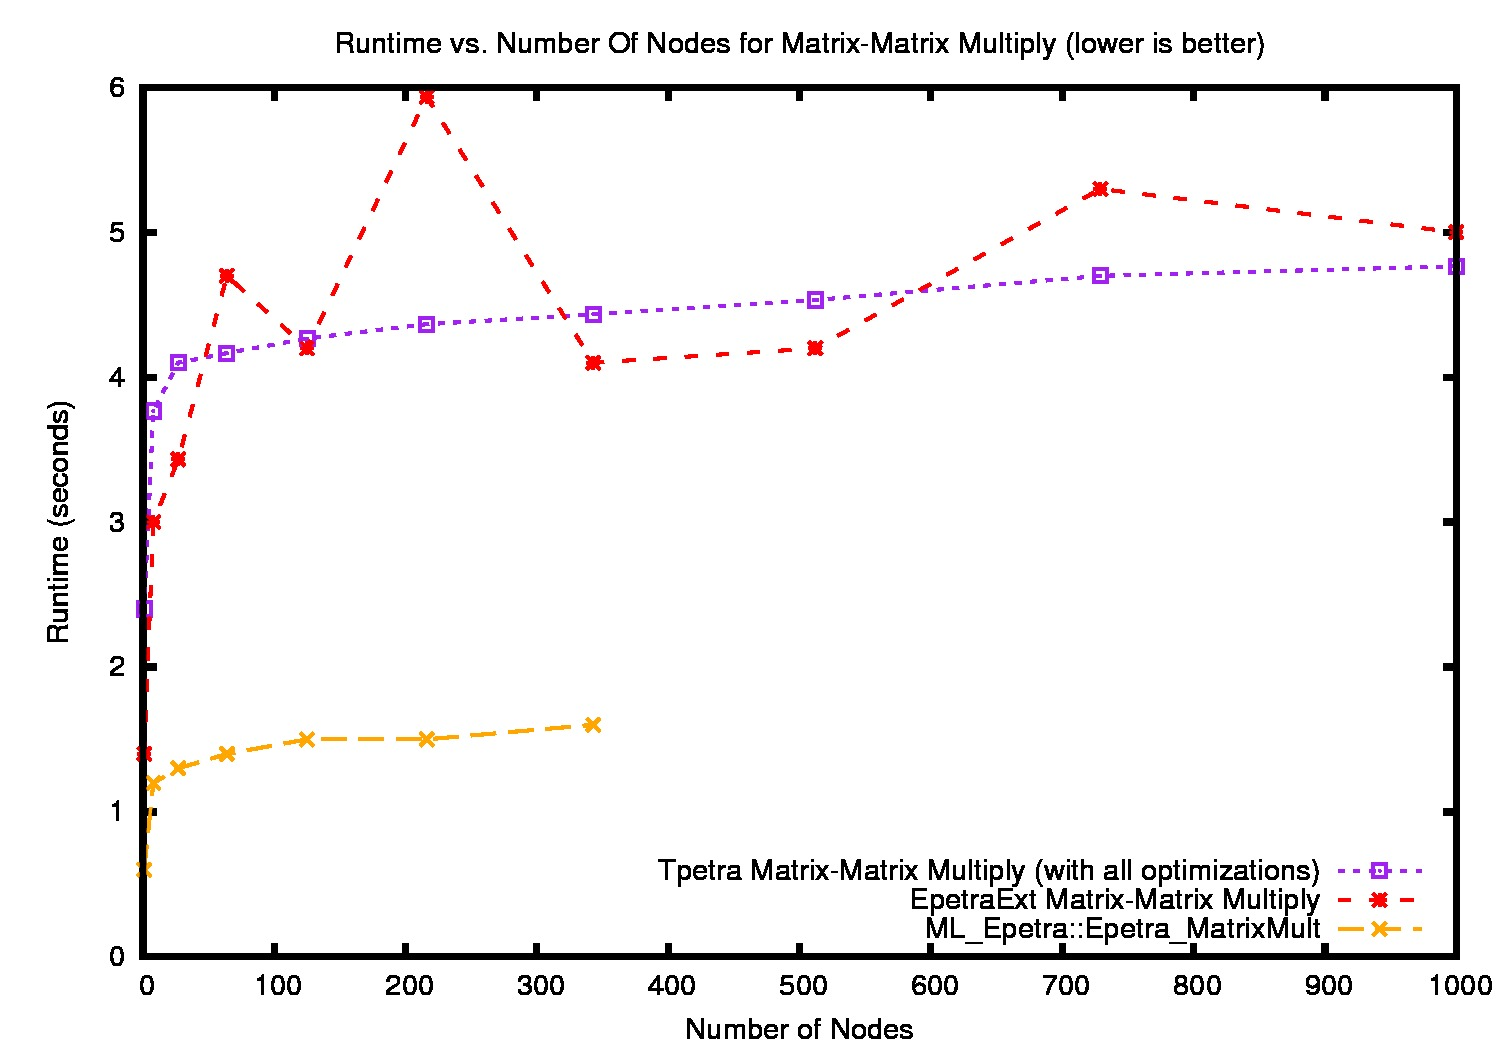
\includegraphics[scale=.4]{totaltime.jpg}
\caption[Time Comparison]{A comparison of various Trilinos matrix multiply routines' runtime}
\label{totaltime}
\end{figure}

\begin{figure}
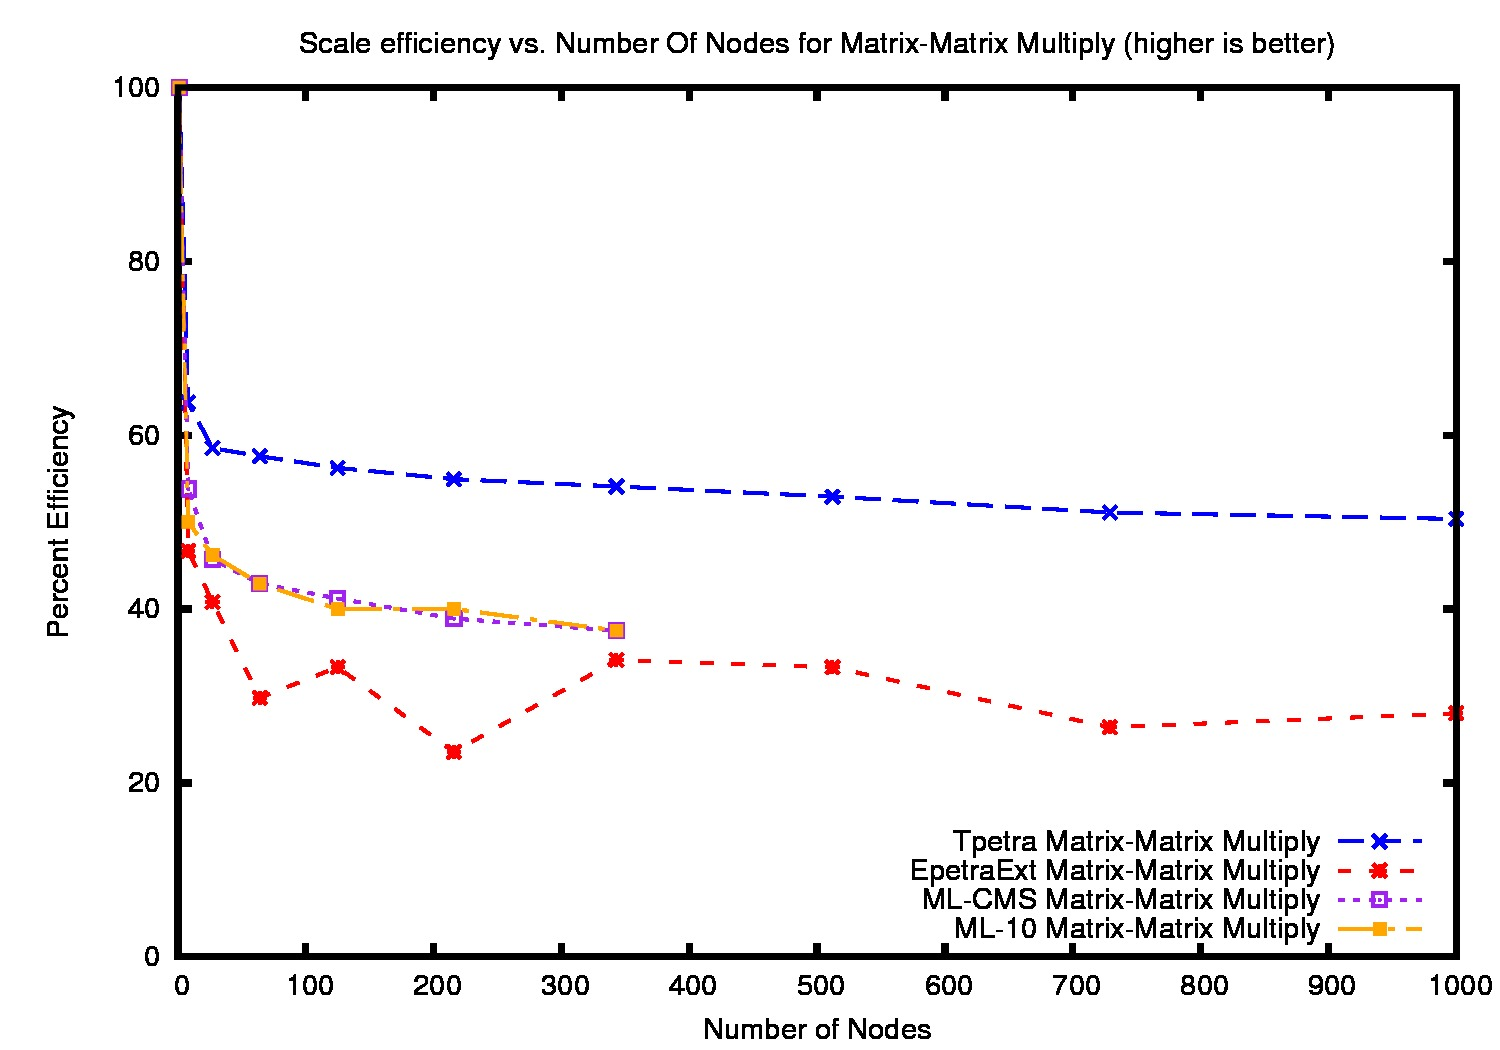
\includegraphics[scale=.4]{totaleff.jpg}
\caption[Efficiency Comparison]{A comparison of various Trilinos matrix multiply routines' scaling efficiency}
\label{totaleff}
\end{figure}

\subsection{Transpose Mode Tests}
Since Tpetra and EpetraExt differ wildly when it comes to transpose modes, we decided to compare the two. We did the same
tesing procedure as in the development stages comparison, except that we requested A be transposed. Figure~\ref{transtime}
and Figure~\ref{transeff} show the results. To say that the Tpetra algorithm scales better than the EpetraExt algorithm
would be a gross understatement. We attempted to conduct a similar experiment where we transposed B instead of A, 
but the EpetraExt algorithm was taking even longer (over ten minutes on a single node of Hopper) and we didn't want to 
waste our limited computing resources. ML is not included in these results because it does not have a transpose mode.
\JJH{ML matrices could be transposed first, however, then multiplied together.  This is basically what Tpetra does with
the rowMatrixTranposer.}

\begin{figure}
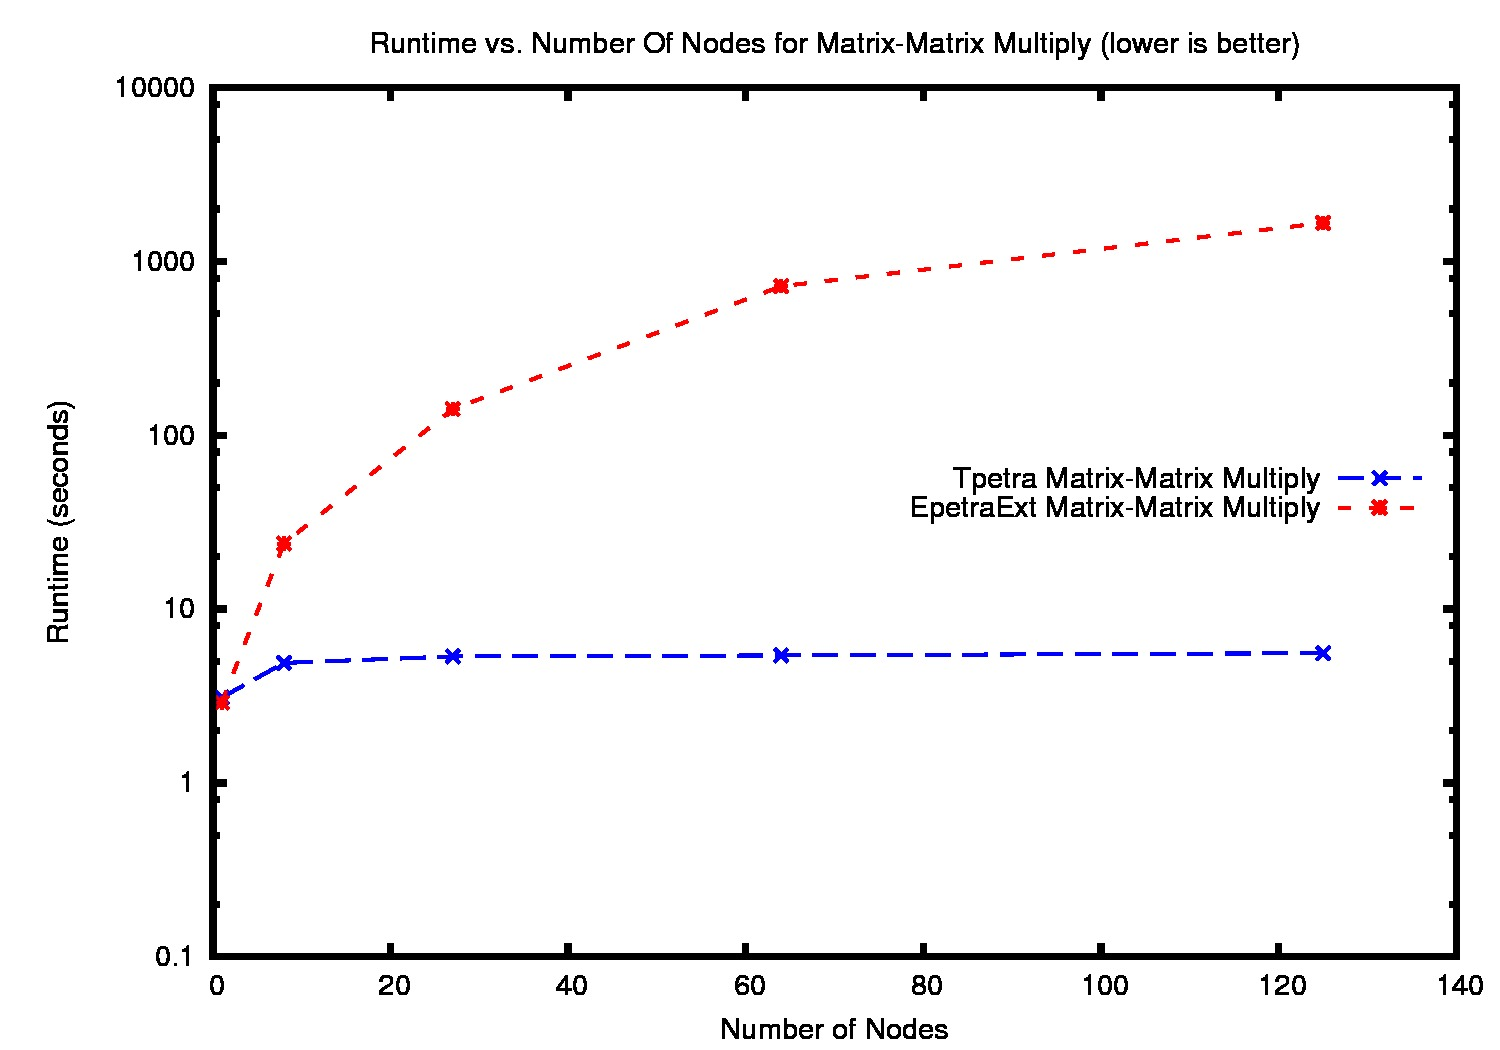
\includegraphics[scale=.4]{atranstime.jpg}
\caption[Time Comparison]{A comparison of matrix matrix multiple runtime in Tpetra and EpetraExt using transpose mode}
\label{transtime}
\end{figure}

\begin{figure}
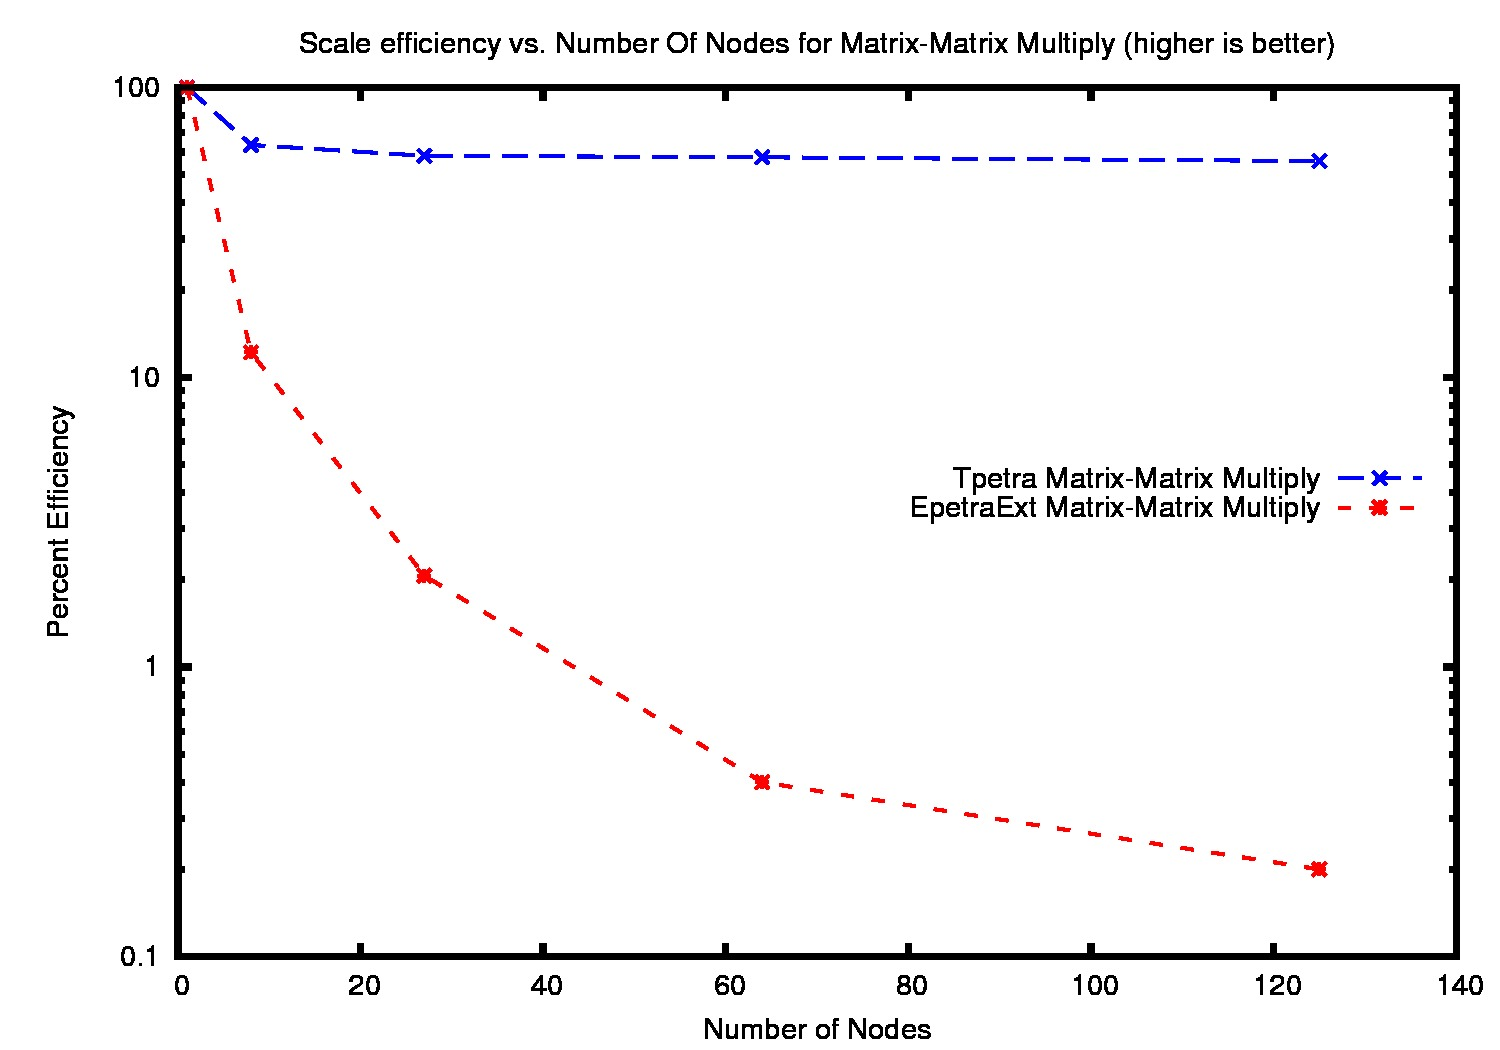
\includegraphics[scale=.4]{atranseff.jpg}
\caption[Efficiency Comparison]{A comparison of matrix matrix multiple scaling efficiencies in Tpetra and EpetraExt using transpose mode}
\label{transeff}
\end{figure}

\section{Areas for Future Improvement}
\subsection{Improvement of Underlying Tpetra Architecture}
The most important thing that will help the matrix multiply routine is to improve the underlying Tpetra architecture. 
Undoubtedly the inefficient sort2 routine was not the only problem with Tpetra at large. There have been reports from other 
scientists at Sandia that things like the Tpetra Import/Export classes are not running as nearly as fast as their Epetra 
counterparts. These things need to be investigated, and fixed if necessary.

\subsection{Kokkos Kernel}
The actual computation kernel should be moved down into Kokkos where it can better take advantage node-parallelism. 
This should offer non-trivial speedups and not be very difficult to implement.

\subsection{Possible Implementation of ML's Algorithm}
ML has a matrix multiply routine that employs a complex hashing scheme in order to speed up lookup times for 
column indices. ML's matrix matrix multiplication algorithm is fast, but it's not clear to the current Tpetra developers 
how much the hashing scheme has to do with ML's speed. That said, it is definitely worth investigating. ML's hashing scheme 
is complex. Figure~\ref{hashalgo} outlines in pseudo code the algorithm as current Tpetra developers 
understand it. While maybe not as easy as implementing a Kokkos kernel, this shouldn't be that difficult to write.

\begin{figure}
\centering
{\footnotesize
\begin{verbatim}
1. For matrix B only, create a hashtable where given a globalid, 
we get a unique hashtag. i.e. hash[gid] = hashtag
Note that in Serial we don't actually need a "hash", local id's should suffice
2.Create a "reverse" map, one where we can do rmap[hastag] = gid
3. Allocate an array called acc_index with the same size as the hash table
4. Allocate two arrays called acc_col and acc_val whose size is 
equal to the maximum number of row entries in matrix A.
5. For each row i in A{
  acc_index.fill(-1)
  ArrayView cur_A_cols;
  ArrayView cur_A_vals;
  A->getRowView(i, cur_A_cols, cur_A_vals);
  curr_acc_ptr=0;
  for each column k in row A[i]{
    ArrayView cur_B_cols;
    ArrayView cur_B_vals;
    (B or Bimport)->getRowView(k, cur_B_cols, cur_B_vals);
    for(j=0; j< cur_B_cols.size(); ++j){
      cur_acc_index = hashtable(getGlobalElement(cur_B_cols[j])) //precomputing this might be useful
      if(acc_index(cur_acc_index) == -1){
        acc_col[cur_acc_prt] = cur_acc_index  //Probably should just put in gid actually
        acc_val[cur_acc_ptr] = cur_B_vals[j]*cur_A_vals[k]
        acc_index[curr_acc_index]=cur_acc_ptr++
      }
      else{
        acc_val[acc_index(cur_acc_index)] += cur_B_vals[j]*cur_A_vals[k]
      }
    }
  }
  c.insertGlobalVals(i, (Global_ids_of_hashes(acc_col))(0, curr_acc_ptr), acc_val(0,cur_acc_ptr))
}

\end{verbatim}
}
\caption[Hash based algorithm]{ML's hash based algorithm for matrix matrix multiply}
\label{hashalgo}
\end{figure}

\end{document}

